\documentclass[11pt]{article}
\usepackage{fullpage}
\usepackage{graphicx}
\usepackage{sidecap}
\usepackage[export]{adjustbox}
\usepackage{amsmath}
\usepackage{wasysym}
\usepackage{hyperref}
\usepackage{comment}
\usepackage{pdfpages}
\usepackage[section]{placeins}
\hypersetup{colorlinks=true, linkcolor=blue, bookmarks=true}

\newtheorem{remark}{Remark}
\newtheorem{example}{Example}
\newcommand{\eat}[1]{}
\begin{document}



\title{Web Information Retrieval (67782)\\ Ex2: Index Construction}
\date{}

\maketitle
\noindent {\bf Submitted by: Daniel Kerbel (CSE: danielkerbel, ID: DELETED)}

\section{Index creation runtime}

The computer which was used has the following specifications:

\begin{itemize}
	\item OS: Windows 10 64-bit
	\item CPU: Intel i5-7300 HQ at 2.5-3.5GHz
	\item RAM: 24GB of RAM, only allocated 1GB to the Java process
	\item Storage: The data-set was stored on a 7200 RPM external hard drive
\end{itemize}

The dataset is the entire \href{https://snap.stanford.edu/data/web-Amazon.html}{1995-2013 Amazon Dataset} (the \texttt{all.txt} file) 
which has the following statistics:

\begin{description}
	\item[Number of products] 34,686,770
	\item[Raw size] 35,781,618,251 bytes
	\item[Total amount of tokens] 2,909,591,866
	\item[Number of unique tokens] 413,742,857
\end{description}

I've also tested a few smaller datasets which are included in this file.

Index creation was implemented using the SPIMI(merge based) algorithm, and I've split the measurement into two stages:

\begin{itemize}
	\item Time taken by the "invert" stage (including parsing), where many temporary indices are created
	\item Time taken to merge all indices and create the final index
\end{itemize}


\hyperref[fig:cumruntime]{Click here} to see the number of tokens processed as function of time, for each data-set

\hyperref[fig:totalruntime]{Click here} to see the total time as function of the total reviews.


\begin{SCfigure}[1][!htb]
	\centering
	\caption{Cumulative index construction time at various stages, plot for each dataset.
	\\\hspace{\textwidth}
	The invert stage also included IO for filling the "compact storage" which includes reviews metadata (which is just filled sequentially as
	we encounter new documents, and doesn't require any sorting or special processing).
	Not included is the time taken to sort productID - docID pairs, containing the lowest \& highest review IDs per product.
	I've actually implemented this via an external sorting algorithm, but as it turns out, only 1 block was needed(the sort was performed entirely within memory), and finished in a couple seconds.
	}
	\label{fig:cumruntime}
	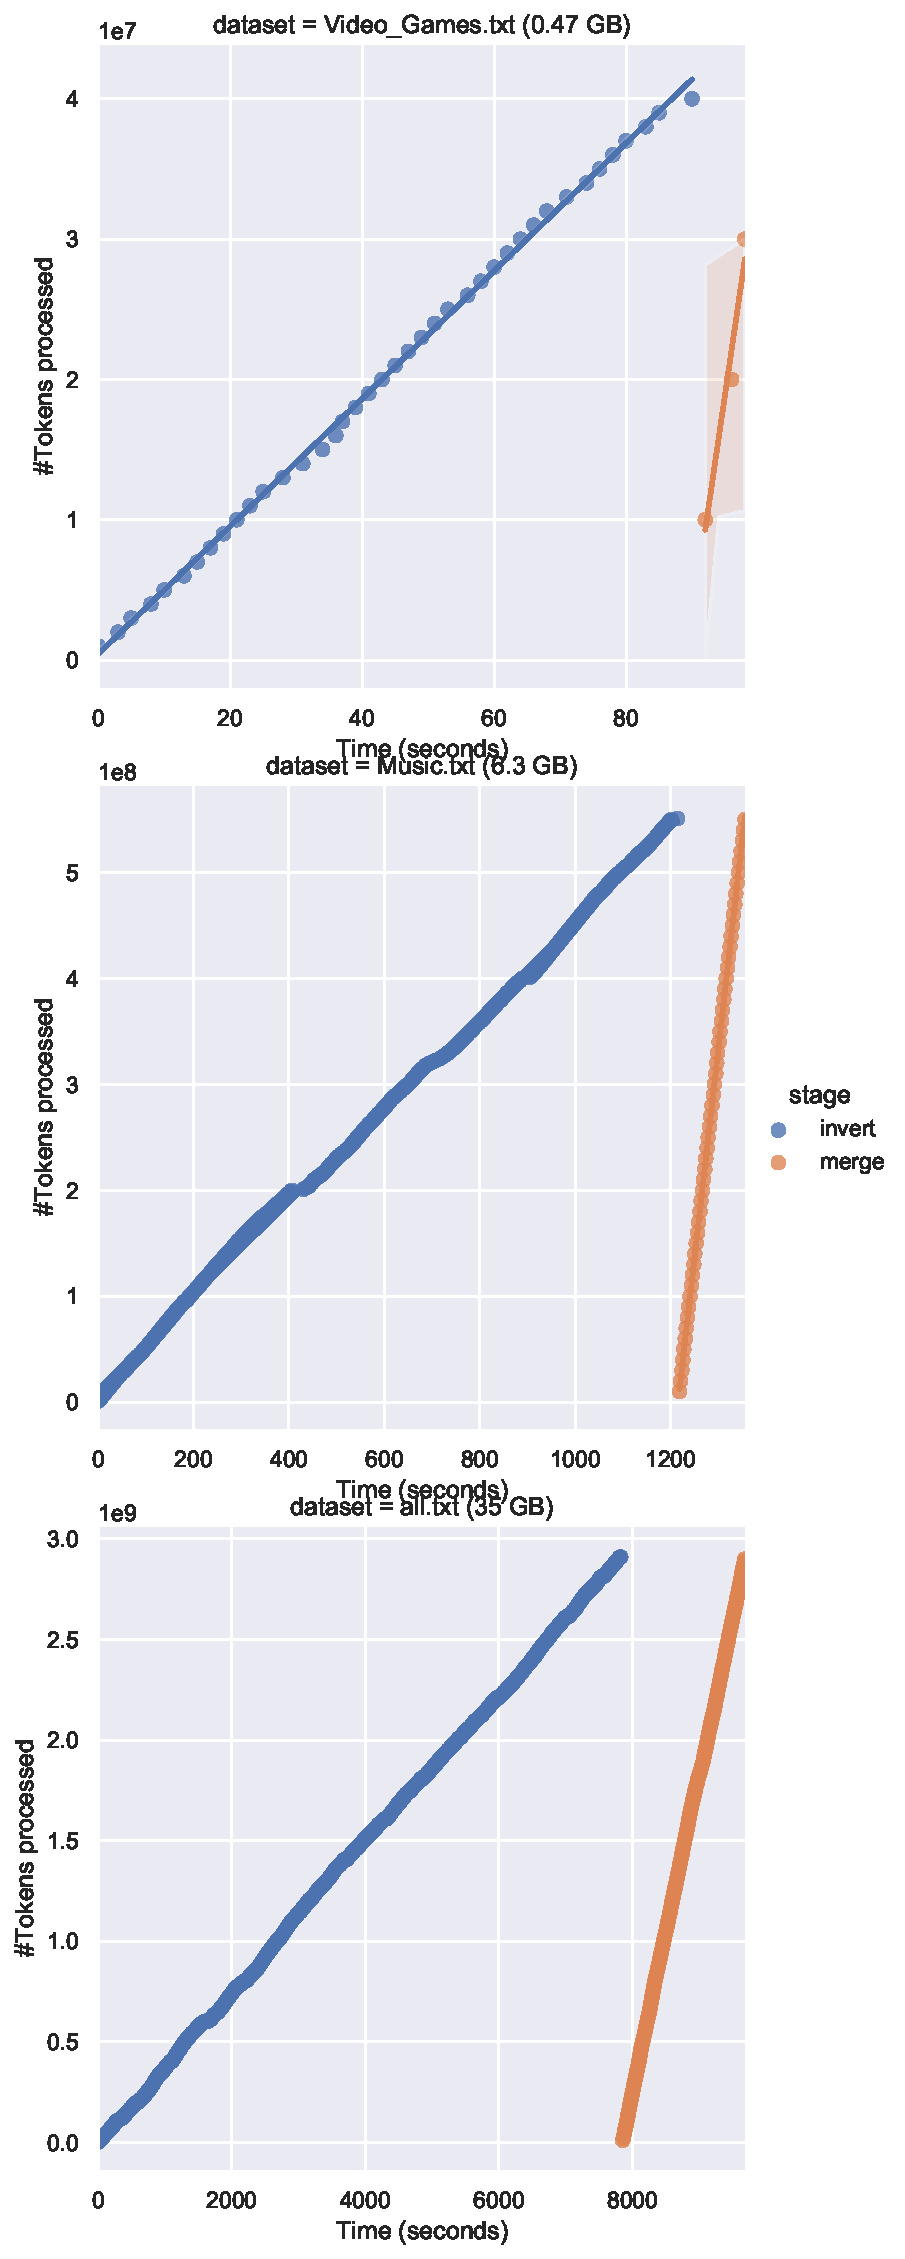
\includegraphics[width=\textwidth,height=\textheight,keepaspectratio]{runtime.pdf}
\end{SCfigure}


\begin{figure}[!htb]
	\caption{Total index construction running time}
	\label{fig:totalruntime}
	\centering
	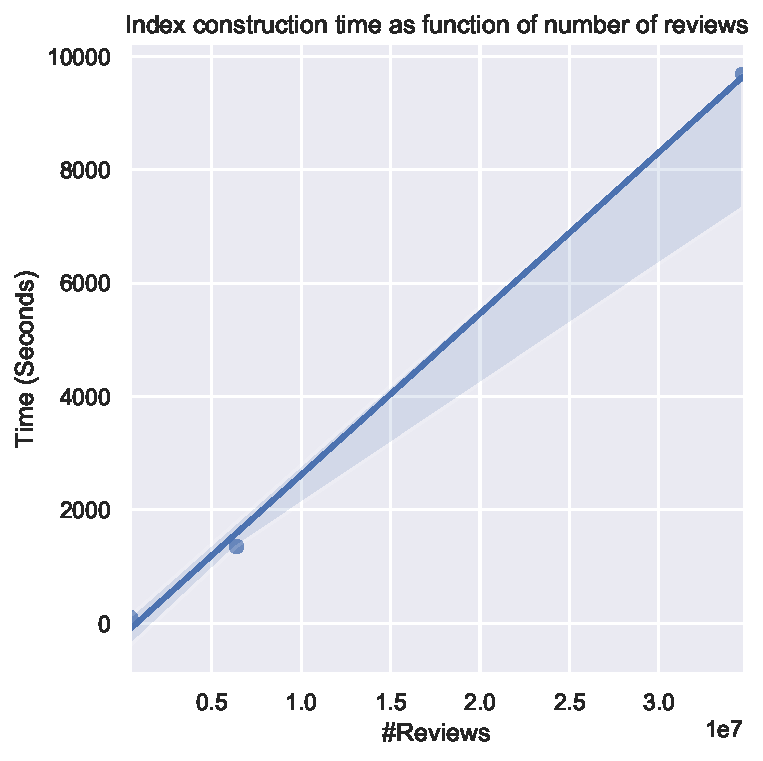
\includegraphics[width=\textwidth,height=\textheight,keepaspectratio]{runtime2.pdf}
\end{figure}




\section{Disk usage}

During the invert stage of \textbf{all.txt}, 15 temporary indices were created, each taking around ~540 MB, and using a total of 8 GB. In addition
to the original dataset of 35 GB, this means we need a total disk usage of 43 GB, which implies a $22\%$ disk size overhead during index construction.
\footnote{In theory, we could use something similar to 8 GB if we split the input file, and remove splits that we're processed, as we only go over the input once}

\hyperref[fig:cumsize]{Click here} to see temporary index size(not final) for each dataset, as a function of time

\hyperref[fig:finalsize]{Click here} to see the final index size, as a function of total reviw count.

After merging, the final index takes \textbf{8.46 GB}. This means that during merging, we use a total of 16.46 GB (adding up the temporary and final indices, but omitting the input files as they aren't needed at this point)

\begin{figure}[!htb]
	\caption{Cumulative temporary index size(not final) over time}
	\label{fig:cumsize}
	\centering
	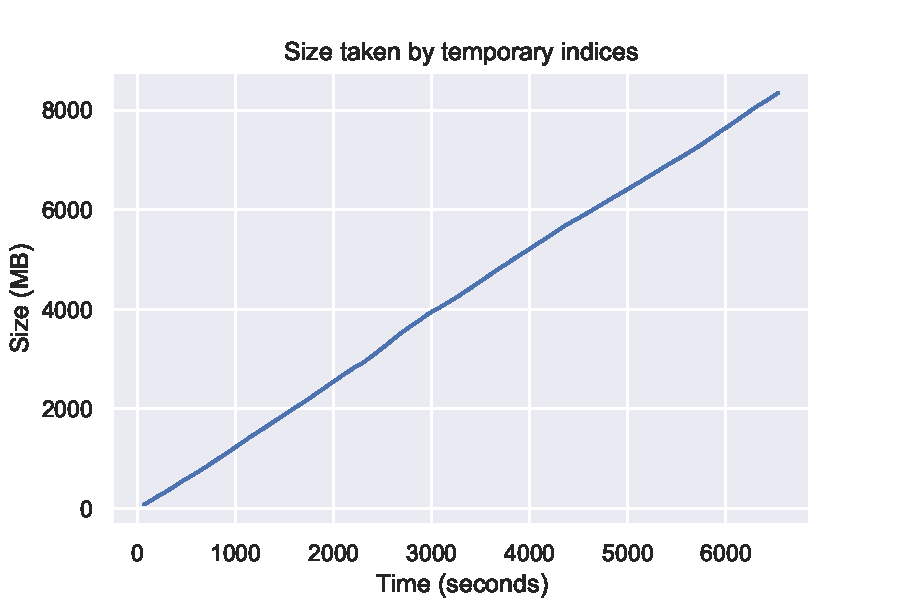
\includegraphics[width=\textwidth,height=\textheight,keepaspectratio]{diskusage.pdf}
\end{figure}

\begin{figure}[!htb]
	\caption{Final index size(not counting temporary or input files)}
	\label{fig:finalsize}
	\centering
	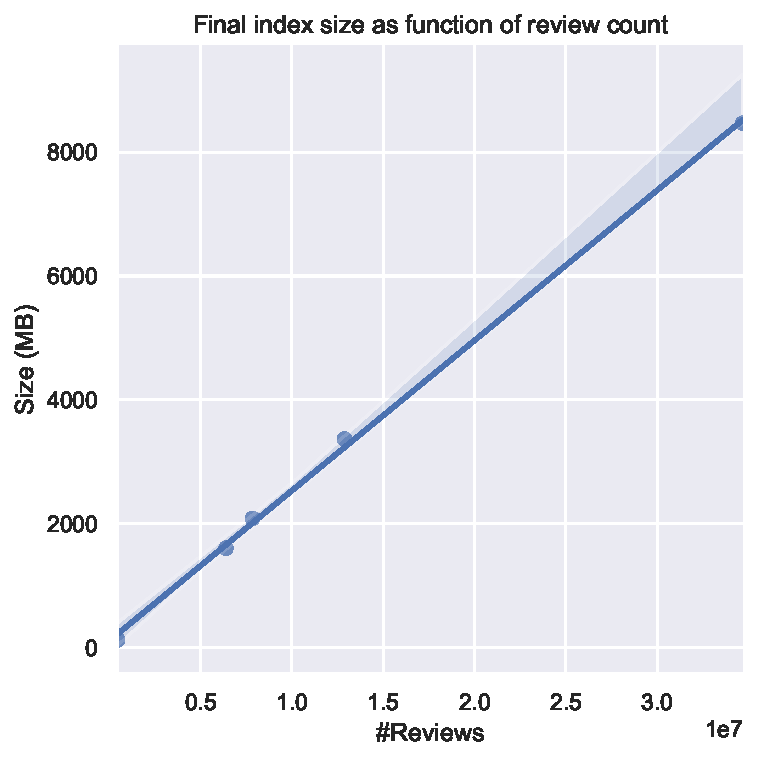
\includegraphics[width=\textwidth,height=\textheight,keepaspectratio]{diskusage2.pdf}
\end{figure}

\section{Index query operations}

For each of the previous data-sets, I've measured the total time to perform 100 requests to \texttt{getReviewsWithToken} or \texttt{getTokenFrequency}, by using 100 terms chosen independently and uniformly from the entire set of tokens in the dataset.(Chosen for each data-set before timing began). It should be noted that I take a random subset of terms, and not tokens, so terms that appear frequently do not have a higher chance of being picked.


The resulting plot can be seen \hyperref[fig:ops]{here}. I've repeated the same same test a couple of times, each time with different
randomly chosen tokens - this can be visualized by several points of the same color within the same vertical line(same data-set). 



\begin{itemize}
	\item \texttt{getTokenFrequency} has a logarithmic time complexity, this can be observed from the plot due to the fact that the running time increases much slower than the increase
	in the number of reviews, in fact the running time is nearly constant aside from an outlier. This makes sense considering it is performing binary search within main memory.
	
	\item \texttt{getReviewsWithToken}, which includes time for iterating the enumeration, is slower by about 2 orders of magnitude than the above due to the disk IO while iterating over posting lists. The trend appears linear but there's an outlier for one of the review sizes. The running time is affected by 2 factors:
	\begin{itemize}
		\item Time taken to find the posting list pointer within
		the dictionary via binary search, which is logarithmic.
		\item Time taken to iterate over the posting lists. On the one hand, as we increase the review size, the posting lists of common terms get longer(a linear increase in the iteration running-time), on the other hand, the vocabulary size increases, and rarer terms have shorter posting lists.
		
		Overall, the former case seems to be more dominant, explaining the linear trend, but one of the reviews is an outlier, which is explained by a richer vocabulary, with shorter posting lists per term.
	\end{itemize}
\end{itemize}



\begin{figure}[!htb]
	\caption{Index query running times}
	\label{fig:ops}
	\centering
	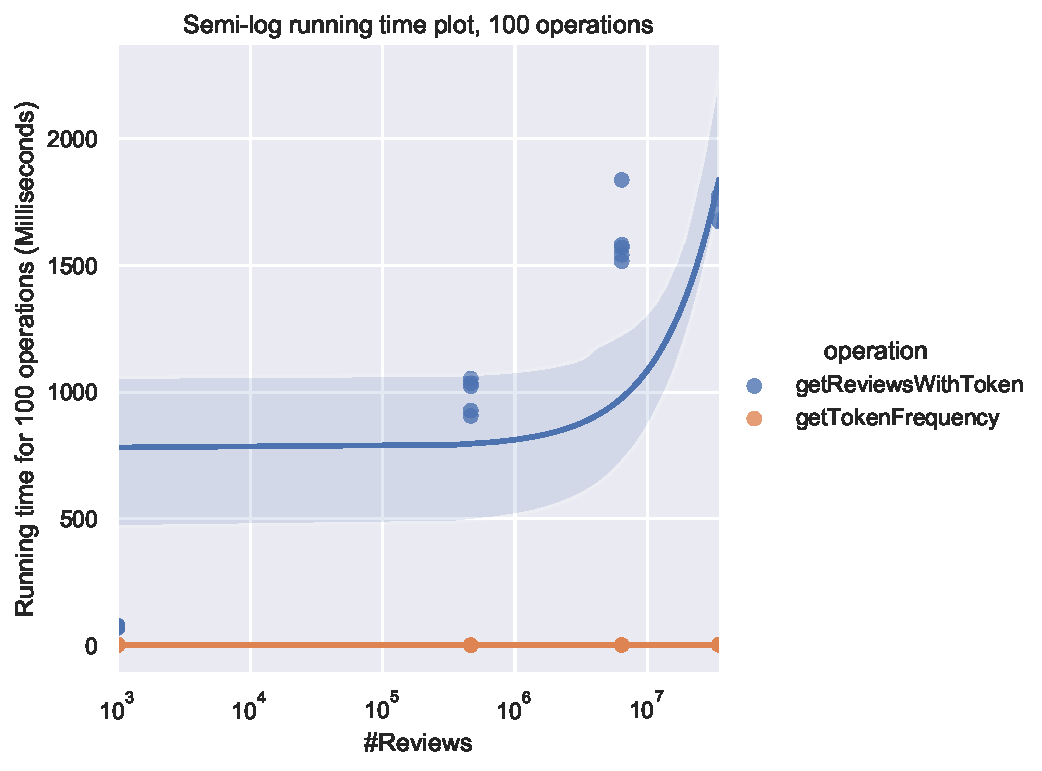
\includegraphics[width=\textwidth,height=\textheight,keepaspectratio]{ops.pdf}
\end{figure}


\end{document}
